%!TEX root = ../thesis.tex

\section{ルールベース制御器で用いる装置}

  本研究で用いた2DLiDARは北陽電気社製のUTM-30LX\cite{hokuyo}である.これは,ROS上で\texttt{urg\_node}\cite{urg_node}というパッケージが提供されており,インストールするだけで簡単にデータのやり取りができる.データは,物体までの距離情報だけでなく,物体の反射強度の値も取得できる2DLiDARである.基本的には,\texttt{urg\_node}で提供されているデフォルトのパラメータを使用するが,\tabref{tab:parameters_of_urg_node}に示すようにパラメータを一部変更している.このセンサ自体の最大検出範囲は270 \,[deg]であるが,反射強度モードを使用する際に最大検出範囲を120 \,[deg]に制限することが推奨されている\cite{urg_node}.そのため,センサの正面を0 \,[deg]としたときに,左側に60 \,[deg](1.047 \,[rad]),右側に-60 \,[deg](-1.047 \,[rad])の最大120 \,[deg](2.094 \,[rad])とした.また,1回のスキャンは25 \,[ms]かかり,-60 \,[deg]から0 \,[deg]を通り60 \,[deg]に向かってレーザーが回転する.このイメージを\figref{Fig:Image of scan}に示す.

  \begin{table}[hbtp]
    \caption{Parameters of \texttt{urg\_node}}
    \label{tab:parameters_of_urg_node}
    \centering
    \begin{tabular}{|c|c|c|}
    \hline
    Parameter   & Default & After change \\ \hline
    intensities & false   & true         \\ \hline
    angle\_min  & -       & -1.047       \\ \hline
    angle\_max  & -       & 1.047        \\ \hline
    \end{tabular}
    \end{table}

    \begin{figure}[h]
      \centering
      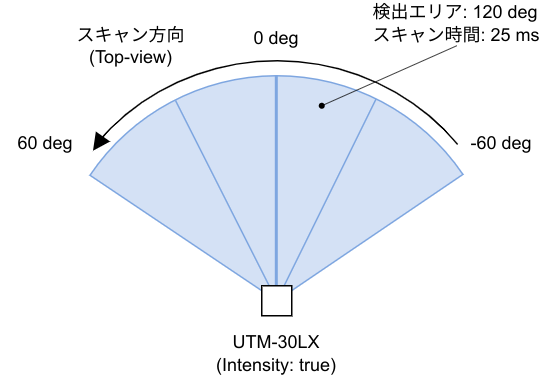
\includegraphics[keepaspectratio, scale=0.40] {images/RobotGuidance_hokuyo_scan.png}
      \captionsetup{justification=raggedright} % キャプションを左寄せに
      \caption{Image of scan}
      \label{Fig:Image of scan}
    \end{figure}

\newpage